\documentclass[tikz,border=10pt]{standalone}
\begin{document}
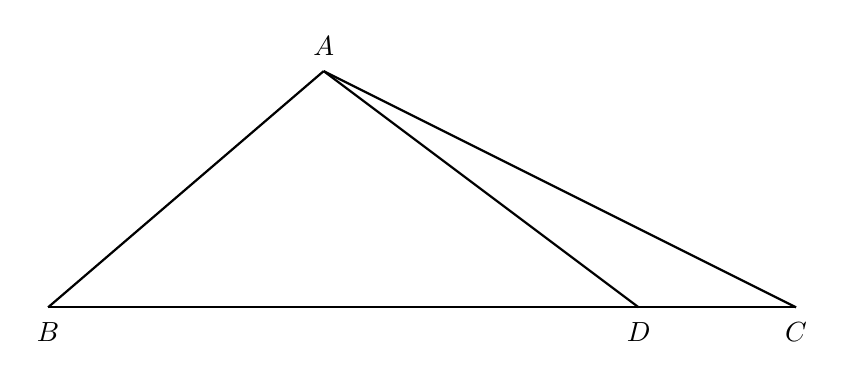
\begin{tikzpicture}
\coordinate (A) at (3.5,3);
\coordinate (B) at (0,0);
\coordinate (C) at (9.5,0);
\coordinate (D) at (7.5,0);

\draw[thick] (B) -- (C);
\draw[thick] (A) -- (B);
\draw[thick] (A) -- (D);
\draw[thick] (A) -- (C);

\node[above=2pt] at (A) {$A$};
\node[below=2pt] at (B) {$B$};
\node[below=2pt] at (D) {$D$};
\node[below=2pt] at (C) {$C$};
\end{tikzpicture}
\end{document}
